\chapter*{Terminology}

\ifnotes

    Learning outcomes:

\fi

\ifcontent

    Some of the challenges that we face are due to misunderstandings that arise from poorly defined terms. We'll be using some words and phrases in this course that are in common use in the software industry. Let's make sure that we have a shared understanding of what they mean:
    
    \begin{itemize}
        \item Acceptance test
        \item Business rule
        \item Cucumber
        \item Example
        \item Product backlog
        \item Programmer test
        \item User story
    \end{itemize}
 
     Discuss with your group which of the definitions in the table below explains each of the terms in the list above.
     
     \begin{center}
        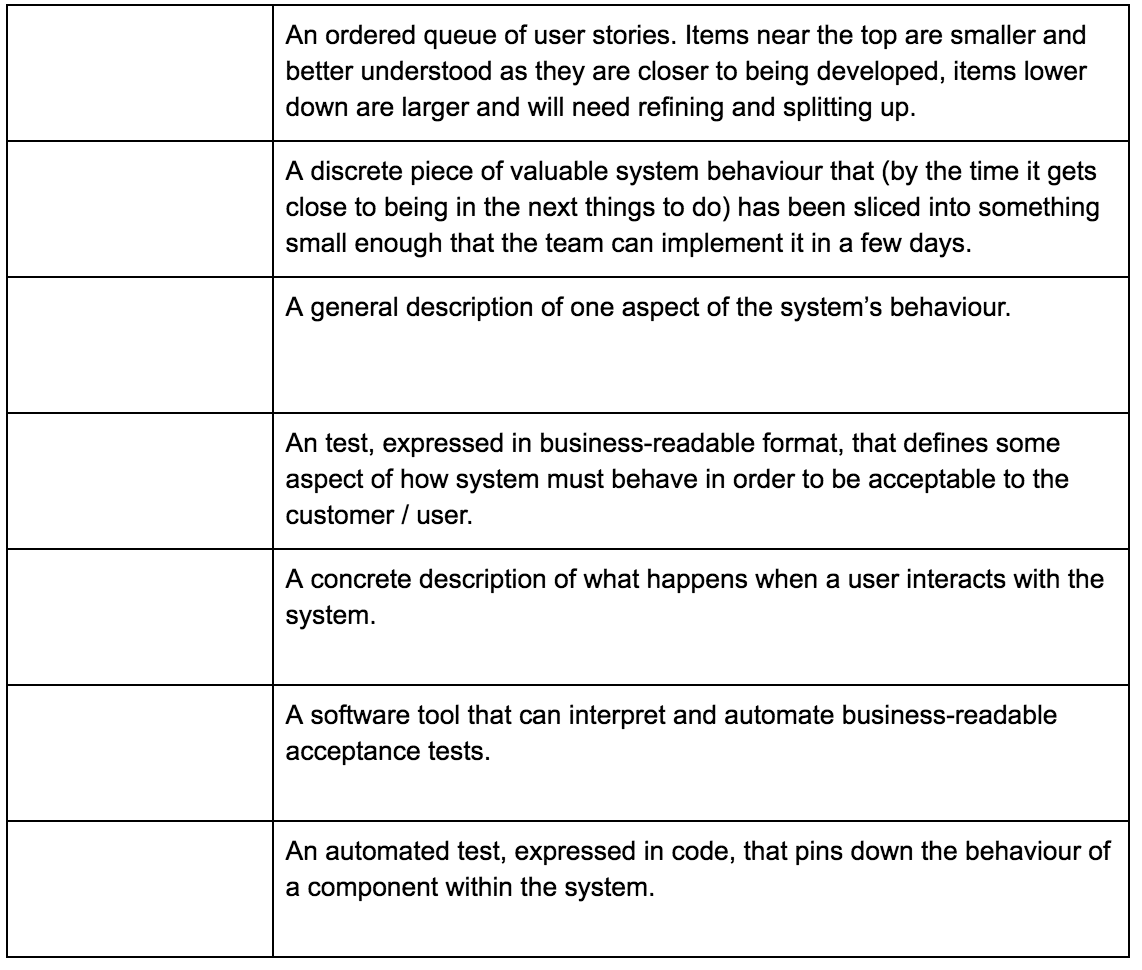
\includegraphics[width=0.9\textwidth]{../bdd-fundamentals/images/terminology-table}
     \end{center}
\fi